\numberedsection{RF5.3 Editar relación}

\subsection*{Descripción}
Permite a los usuarios modificar los datos de las categorías existentes.\par
\vspace{0.15cm}

\textbf{Pre-condición}\par
El usuario ha iniciado sesión en el sistema y se encuentra en el apartado de Gestión de Categorías. La categoría a editar debe existir en el sistema.\par
\vspace{0.15cm}

\textbf{Post-condición}
\begin{itemize}
    \item Caso de éxito: El sistema actualiza los datos de la categoría seleccionada y refleja los cambios en la lista de categorías.
    \item Caso mínimo: El sistema notifica al usuario el resultado de la acción de edición de la categoría: exitosa o fallida.
\end{itemize}

\textbf{Prioridad: }
Media
\vspace{0.15cm}

\textbf{Autor: }
Janine Bernadeth Olegario Laguit\par
\vspace{0.15cm}

\textbf{Control de cambios: } Versión 1: Definición del caso de uso

\numberedsubsection{Escenario principal}
\begin{enumerate}
    \item El usuario accede a la sección de gestión de categorías.
    \item El sistema muestra la lista de categorías existentes y la opción para editar una categoría.
    \item El usuario selecciona la opción de editar una categoría existente.
    \item El sistema presenta un menú con el nombre actual de la categoría.
    \item El usuario ingresa el nuevo nombre para la categoría.
    \item El usuario confirma la modificación del nombre.
    \item El sistema valida el nuevo nombre y actualiza la categoría en la base de datos.
    \item El sistema muestra un mensaje de éxito y refleja el nuevo nombre en la lista de categorías.
\end{enumerate}

\numberedsubsection{Escenarios alternativos}
\begin{description}
    \item[4.a] El usuario cancela la acción de editar la categoría seleccionada.
    \begin{enumerate}
        \item[4.a.1] El sistema regresa a la sección de gestión de categorías sin realizar ningún cambio.
    \end{enumerate}

    \item[6.a] El usuario deja el nombre de la categoría vacío.
    \begin{enumerate}
        \item[6.a.1] El sistema muestra un mensaje de error solicitando un nombre válido.
        \item[6.a.2] El usuario ingresa un nombre válido y confirma nuevamente.
    \end{enumerate}
\end{description}

\numberedsubsection{Casos de Prueba}
\underline{Escenario: Principal}\par
\vspace{0.15cm}

\textbf{Dado} que he iniciado sesión con mi cuenta de usuario correspondiente,\par
\textbf{Y} estoy en el apartado de Categorías,\par
\textbf{Cuando} selecciono la opción de editar una categoría existente,\par
\textbf{Y} el sistema presenta un menú con el nombre actual de la categoría,\par
\textbf{E} introduzco el nuevo nombre para la categoría,\par
\textbf{Y} confirmo la modificación del nombre,\par
\textbf{Entonces} el sistema valida el nuevo nombre,\par
\textbf{Y} el sistema actualiza la categoría en la base de datos con el nuevo nombre,\par
\textbf{Y} el sistema muestra un mensaje de éxito,\par
\textbf{Y} refleja el nuevo nombre de la categoría en la lista de categorías.\par

\vspace{0.20cm}

\underline{Escenario: Alternativo 4.a}\par
\vspace{0.15cm}

\textbf{Dado} que he iniciado sesión con mi cuenta de usuario correspondiente,\par
\textbf{Y} estoy en el apartado de Categorías,\par
\textbf{Cuando} selecciono una categoría para editar,\par
\textbf{Y} selecciono la opción de cancelar la acción de edición,\par
\textbf{Entonces} el sistema regresa a la sección de gestión de categorías,\par
\textbf{Y} muestra la lista de categorías sin realizar ningún cambio en la categoría seleccionada.\par

\underline{Escenario: Alternativo 6.a}\par
\vspace{0.15cm}

\textbf{Dado} que he iniciado sesión con mi cuenta de usuario correspondiente,\par
\textbf{Y} estoy en el apartado de Categorías,\par
\textbf{Cuando} selecciono una categoría para editar,\par
\textbf{Y} dejo el campo de nombre de la categoría vacío,\par
\textbf{Entonces} el sistema muestra un mensaje de error,\par
\textbf{Y} me devuelve al gestor de categorías sin realizar ningún cambio.\par

\vspace{0.20cm}

\numberedsubsection{Bocetos}
\begin{figure}[H]
    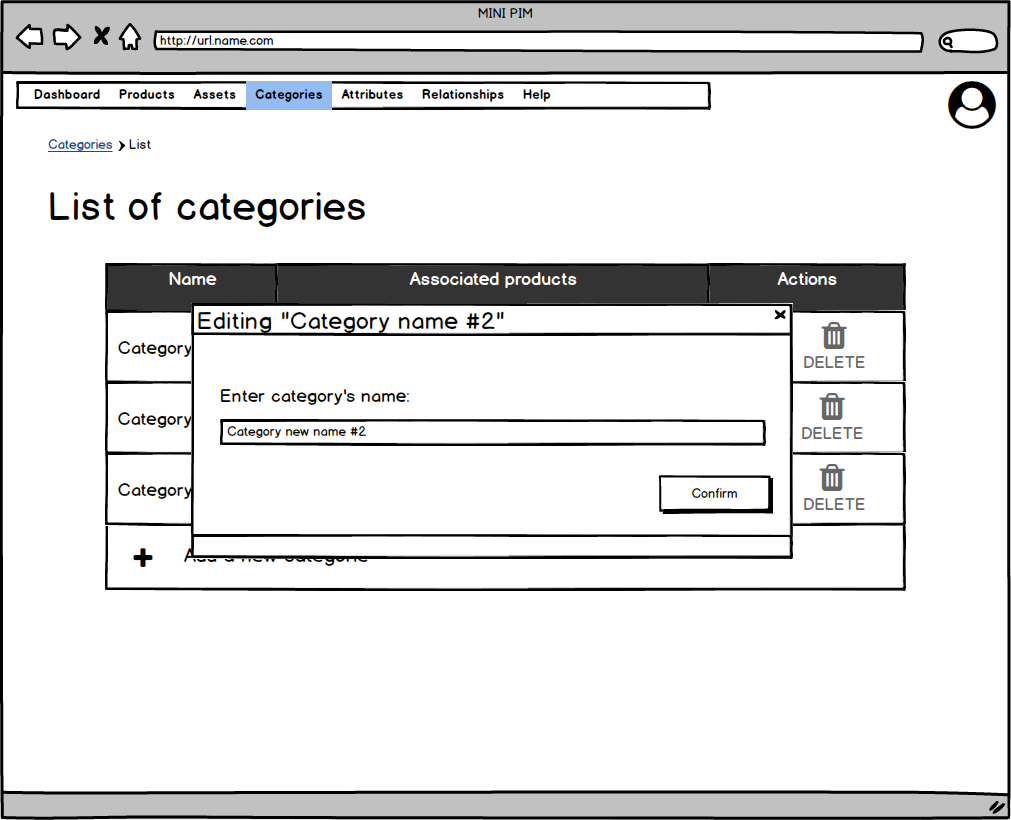
\includegraphics[width=1\linewidth]{mockups/RF4.3_1.png}
    \caption{Editar el nombre de categoría}
   \end{figure}
\vspace{1.0cm}

\begin{figure}[H]
    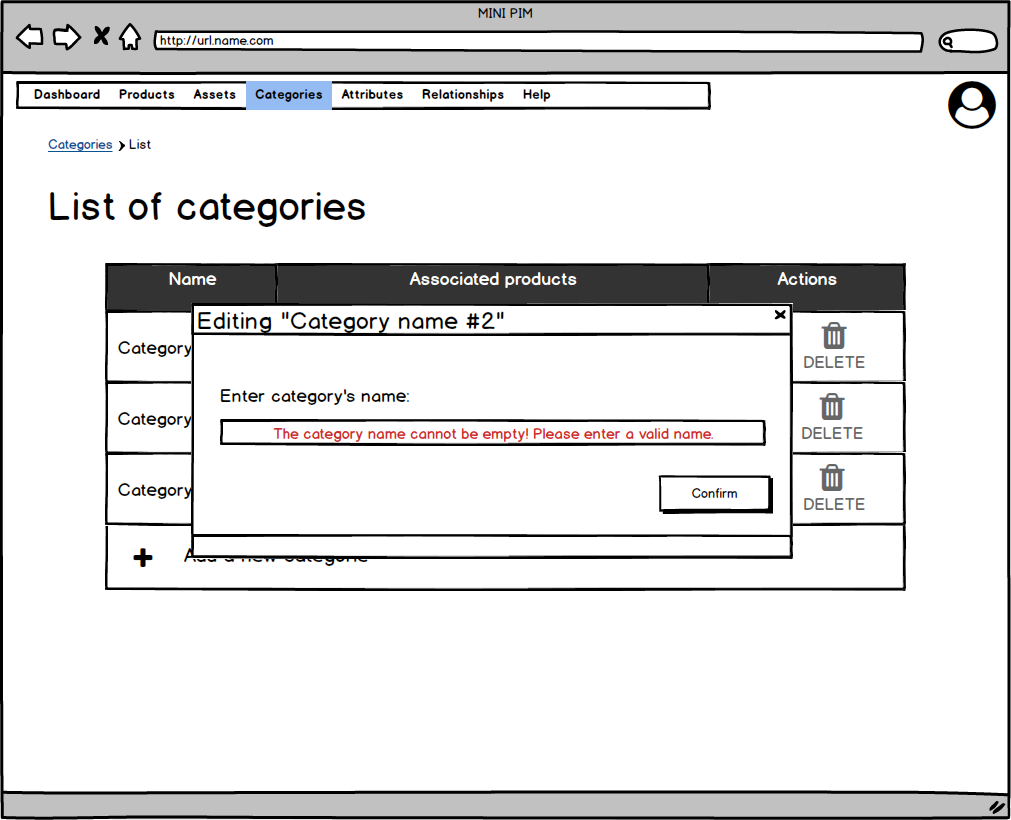
\includegraphics[width=1\linewidth]{mockups/RF4.3_2.png}
    \caption{Error por dejar el nombre vacío}
   \end{figure}
\vspace{1.0cm}

\newpage % Nuevo caso de uso en nueva página